% exercise sheet with header on every page for math or close subjects
\documentclass[12pt]{article}
\usepackage[utf8]{inputenc}
\usepackage{latexsym}
\usepackage{multicol}
\usepackage{fancyhdr}
\usepackage{amsfonts}
\usepackage{amsmath}
\usepackage{amssymb}
\usepackage{enumerate}
\usepackage{listings}
\usepackage{graphicx}
\usepackage[parfill]{parskip}

% Shortcuts for bb, frak and cal letters
\newcommand{\E}{\mathbb{E}}
\newcommand{\V}{\mathbb{V}}
\renewcommand{\P}{\mathbb{P}}
\newcommand{\N}{\mathbb{N}}
\newcommand{\R}{\mathbb{R}}
\newcommand{\C}{\mathbb{C}}
\newcommand{\Z}{\mathbb{Z}}
\newcommand{\Pfrak}{\mathfrak{P}}
\newcommand{\Pfrac}{\mathfrak{P}}
\newcommand{\Bfrac}{\mathfrak{P}}
\newcommand{\Bfrak}{\mathfrak{B}}
\newcommand{\Fcal}{\mathcal{F}}
\newcommand{\Ycal}{\mathcal{Y}}
\newcommand{\Bcal}{\mathcal{B}}
\newcommand{\Acal}{\mathcal{A}}

% formating
\topmargin -3.5cm
\textheight 22cm
\textwidth 16.0 cm
\oddsidemargin -0.1cm

% Fancy Header on every Page
\pagestyle{fancy}
\lhead{\textbf{Embedded Systems Problem Set C}}
\rhead{Daniel Schäfer (2549458)\\ Rafael Dewes (2548365)\\ Kevin M\"uller (2550062)}
\renewcommand{\headrulewidth}{1.2pt}
\setlength{\headheight}{110pt}

\begin{document}
\pagenumbering{gobble}
\lstset{language=C++}

\section*{Problem C1}
I selected the LDF (Latest Deadline First) scheduler to schedule this task with , which results in the following:
\begin{figure}[h]
	\centering
	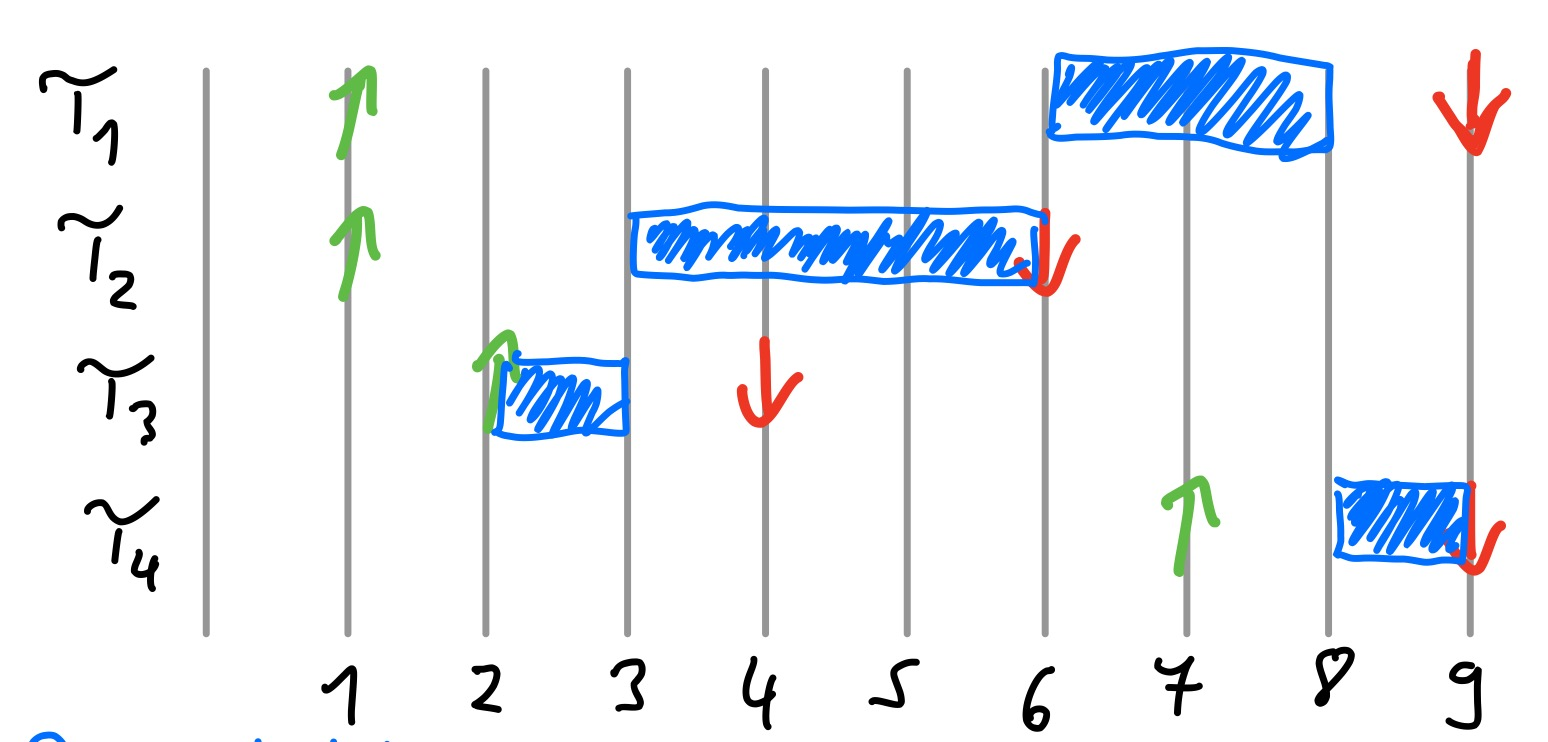
\includegraphics[scale = 0.25]{figures/c1}\\
\end{figure}

\newpage
\section*{Problem C2}
\begin{itemize}
	\item
	  for $\Gamma$ I calculate the Utilization in timeframe $t=12$.
		$$ U = \frac{6 * C(\tau_1) + 2 * C(\tau_2) + 1 * C(\tau_3)}{12} = \frac{11}{12}$$
		\begin{figure}[h]
			\centering
			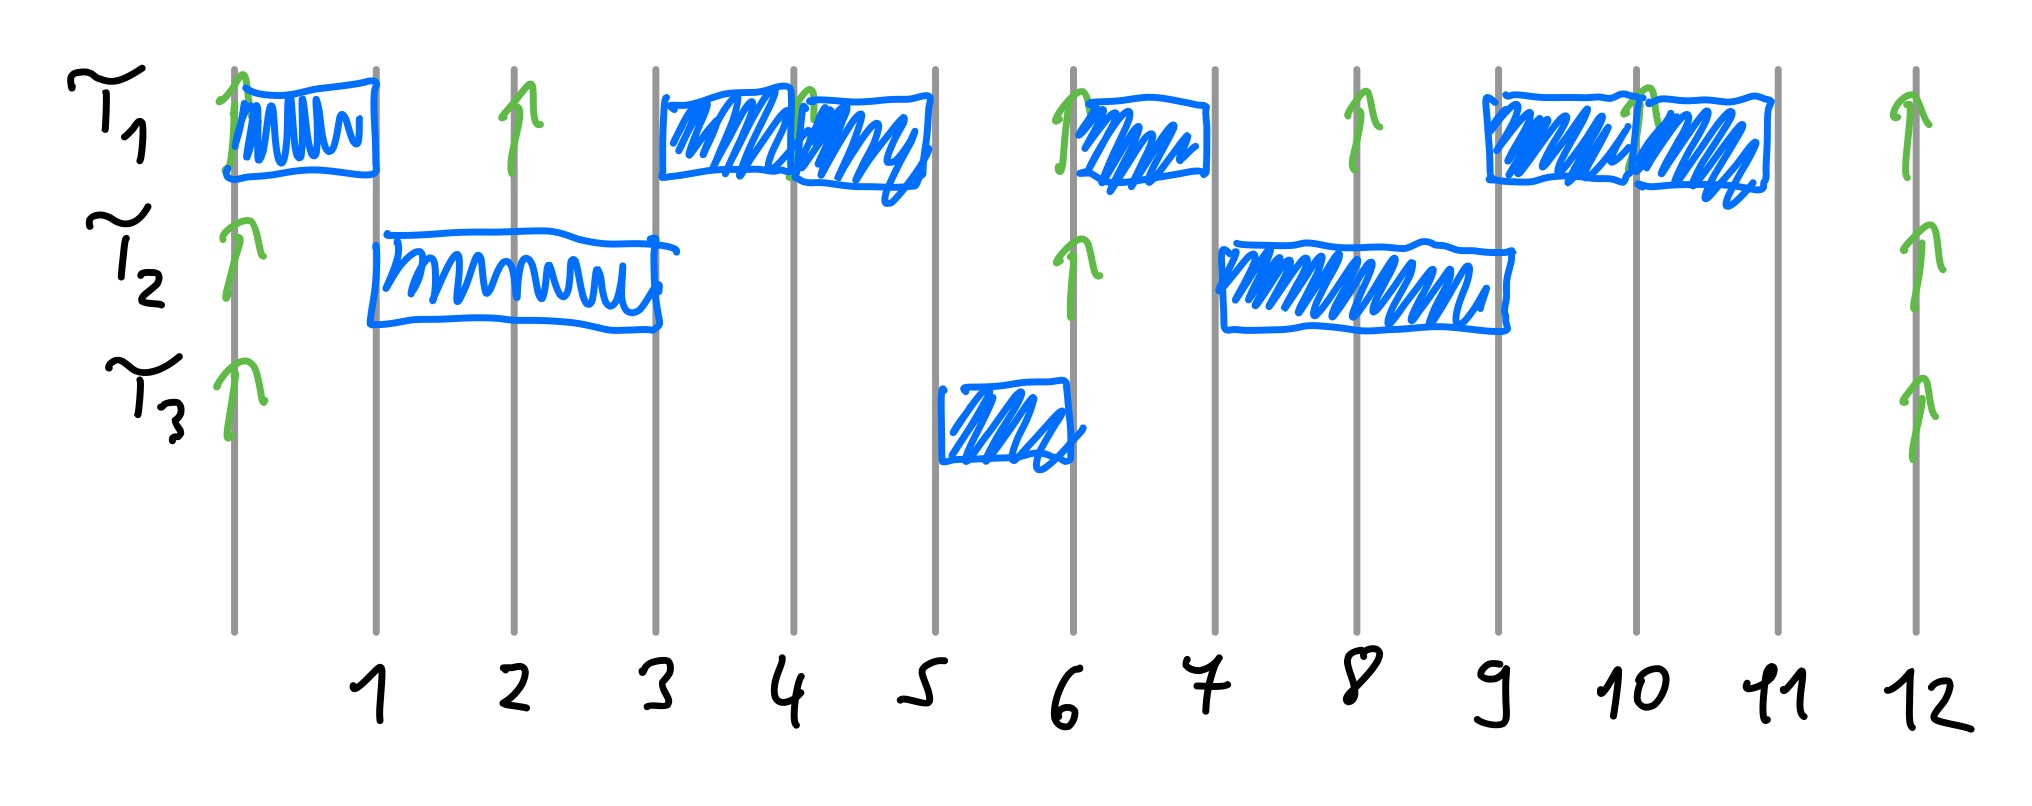
\includegraphics[scale = 0.2]{figures/c2_1}
			\caption{The RM-Schedule for $\Gamma$ for $t=12$}
		\end{figure}

		\begin{figure}[h]
			\centering
			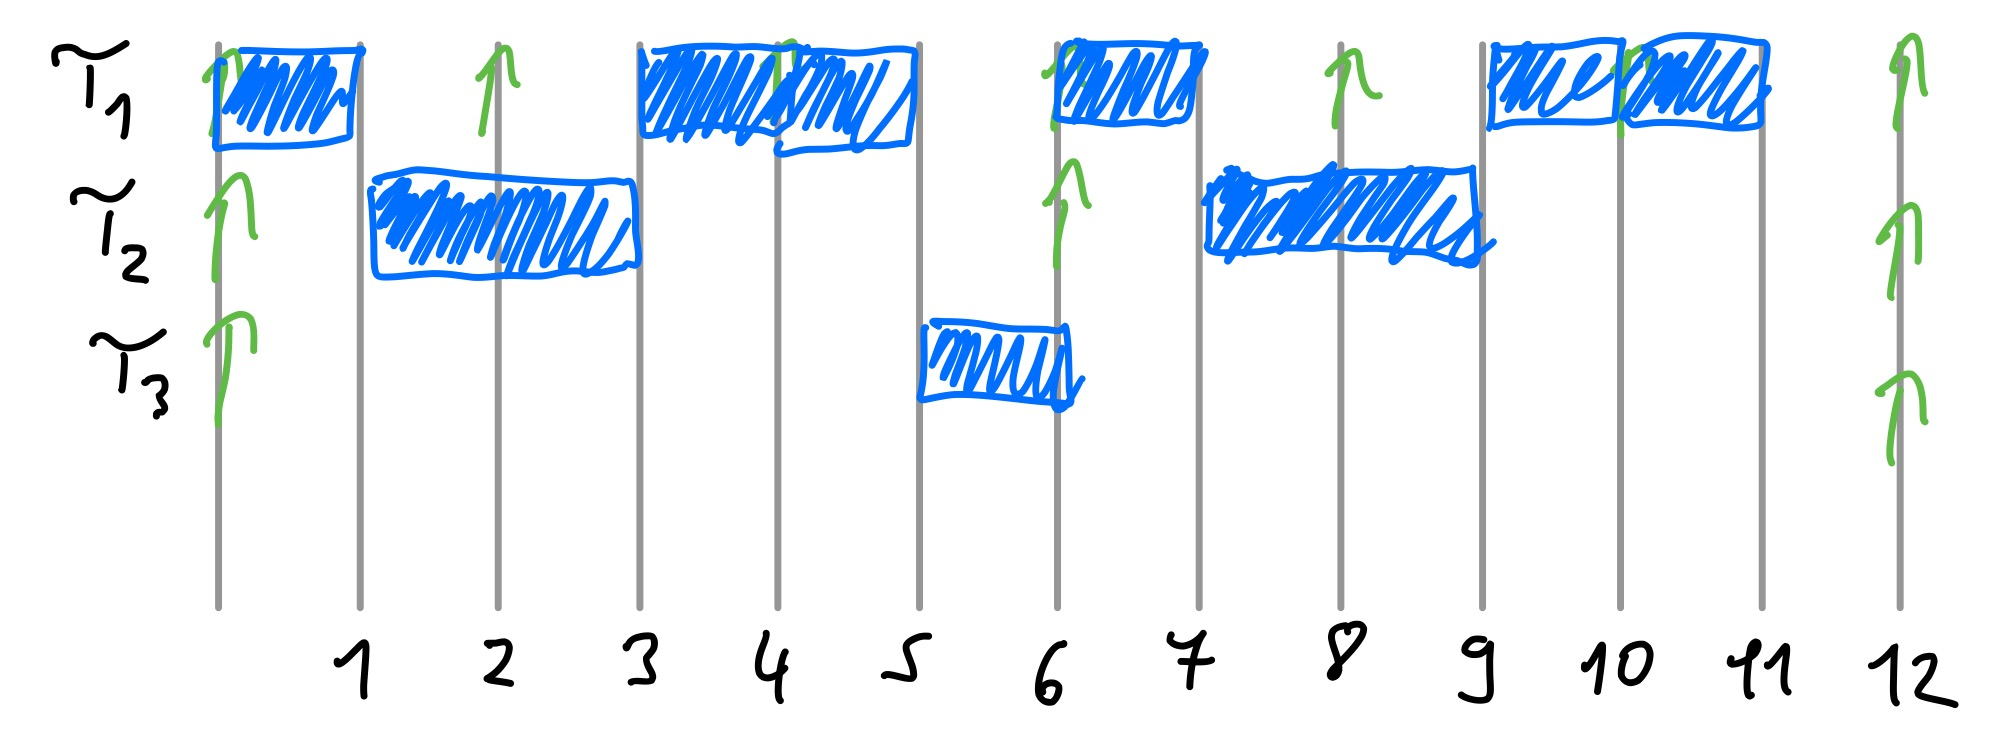
\includegraphics[scale = 0.2]{figures/c2_2}
			\caption{The EDF-Schedule for $\Gamma$ for $t=12$}
		\end{figure}
  \item
    for $\Delta$ I calculate the Utilization in timeframe $t=24$.
		$$U = \frac{1 * C(\tau_4) + 2 * C(\tau_3) + 3 * C(\tau_2) + 4 * C(\tau_1)}{24} = \frac{1 + 6 + 6 + 12}{24} = \frac{25}{24}$$

		Utilization $\frac{25}{24} > 1$, means that this task can not be completed in any scheduler on a single care as it is not feasible.
\newpage
	\item
		for $\Lambda$ I calculate the Utilization in timeframe $t=40$.
		$$U = \frac{1 * C(\tau_4) + 5 * C(\tau_3) + 8 * C(\tau_2) + 20 * C(\tau_1)}{40} = \frac{2 + 10 + 8 + 20}{40} = \frac{40}{40} = 100 \%$$

		\begin{figure}[h]
		\centering
		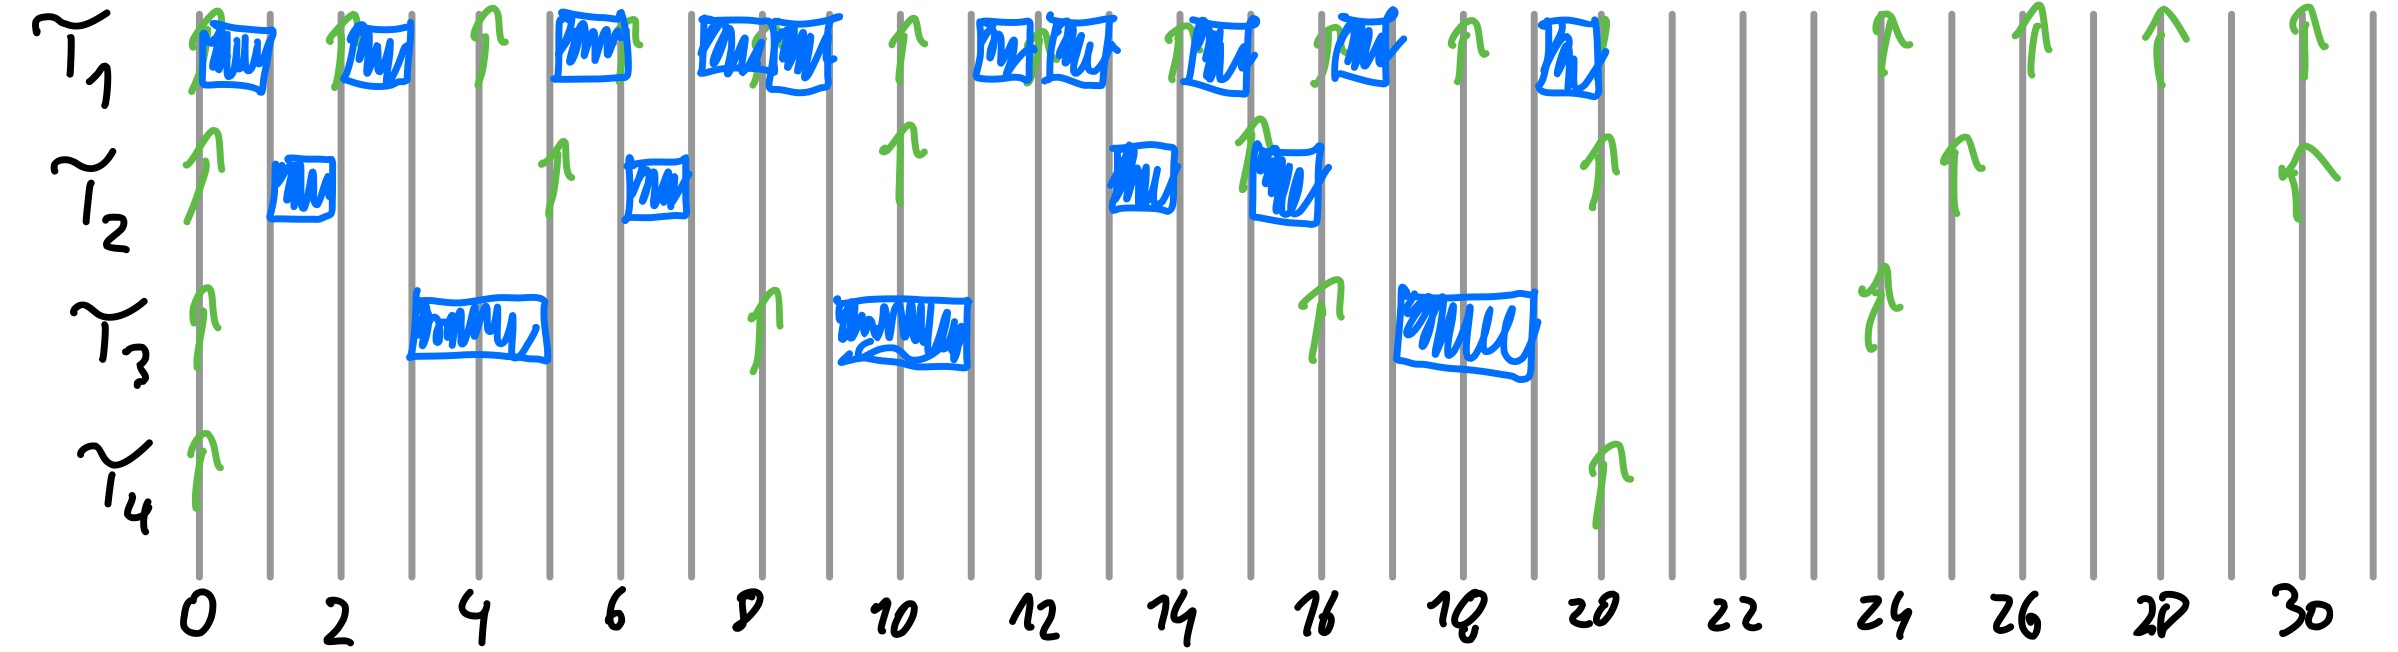
\includegraphics[scale = 0.2]{figures/c2_3}
		\caption{The RM-Schedule for $\Lambda$}
		\end{figure}

		\begin{figure}[h]
		\centering
		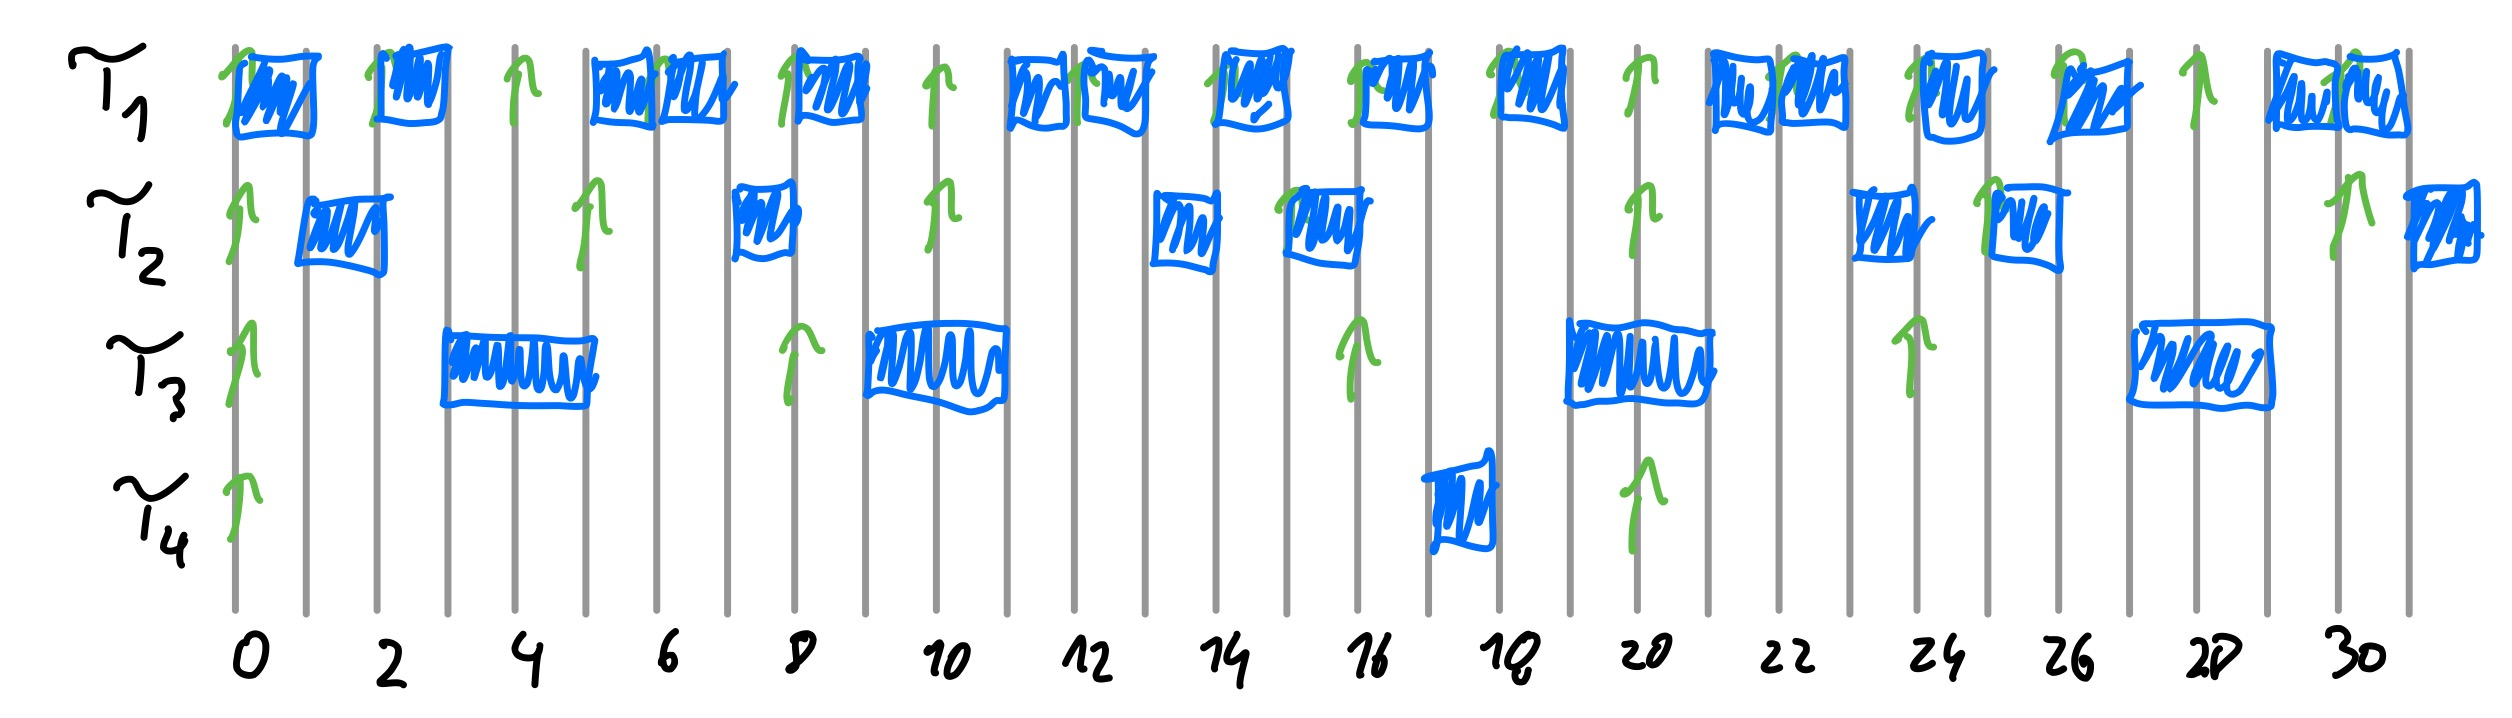
\includegraphics[scale = 0.15]{figures/c2_4}
		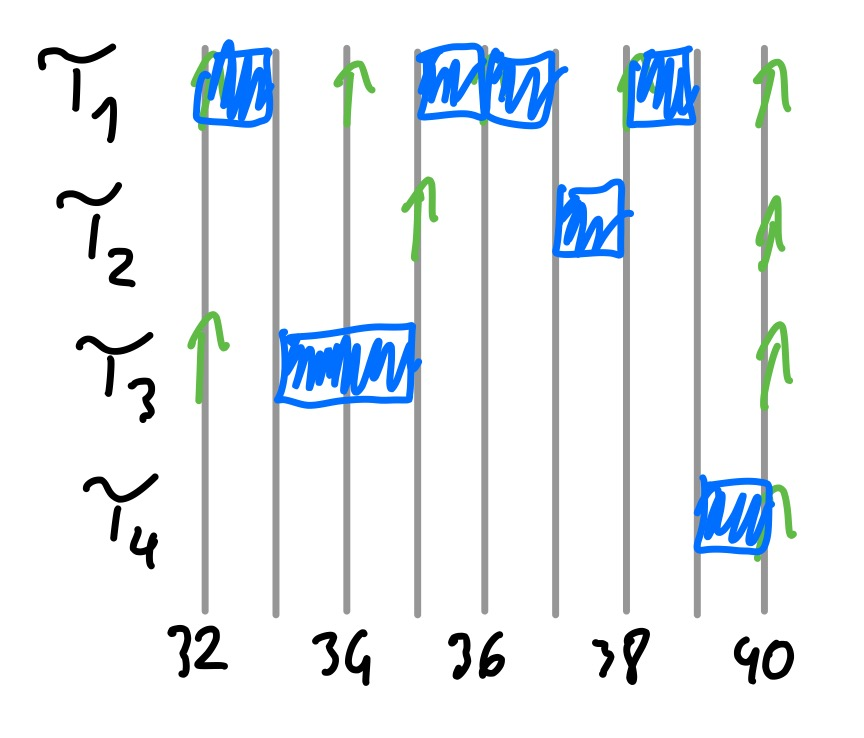
\includegraphics[scale = 0.15]{figures/c2_5}
		\caption{The EDF-Schedule for $\Lambda$}
		\end{figure}
\end{itemize}

\section*{Problem C3}

\subsection*{a)}
We assume a preemptive schedule $\sigma$ with task $J_I$. Assume furthermore $J_I$ being preempted at time $t$ and then resumed at time $t'$ to finish at $f^\sigma_{J_I}$. 

We can remove the preemption of $J_I$ in postponing it by time $t' - t$ so that it still finishes at $f^\sigma_{J_I}$. Call this changed schedule $\sigma'$. All tasks finishing before or starting after $J_I$ in $\sigma$ are unaffected by the change, as is $f^\sigma_{J_I}$. 
Only the tasks running during the preemption of $J_I$ can finish earlier by time $t' - t$, therefore the objective function $T_\omega (\mathcal{J}, \sigma) \geq T_\omega (\mathcal{J}, \sigma')$. 

Removing all preemptions from $\sigma$ in this way yields a non preemptive schedule $\sigma^\star$ with $T_\omega (\mathcal{J}, \sigma^\star) \leq T_\omega (\mathcal{J}, \sigma)$. $\square$

\subsection*{b)}
We presume that a schedule for $\mathcal{J}$ is optimal w.r.t. $T_\omega$ if and only if tasks are sorted in a non increasing order according to their weight $\omega_J$ divided by cost $C_J$.
Assuming two tasks $J_i$ and $J_j$ with $\frac{\omega_{J_i}}{C_{J_i}} < \frac{\omega_{J_i}}{C_{J_i}}$ where $J_i$ finishes at $f^\sigma_{J_i}$ and $J_j$ at $f^\sigma_{J_j} = f^\sigma_{J_i} + C_{J_j}$.
If we switch the execution of these two tasks in the schedule without doing anything else, the value of $T_\omega$ decreases, as:
\begin{align*}
\omega_{J_i} \cdot f^\sigma_{J_i} + \omega_{J_j} \cdot (f^\sigma_{J_i} + C_{J_i}) &> \omega_{J_i} \cdot (f^\sigma_{J_i} + C_{J_j}) + \omega_{J_j} \cdot (f^\sigma_{J_i} + C_{J_j} - C_{J_i} ) \\
\omega_{J_i} \cdot f^\sigma_{J_i} + \omega_{J_j} \cdot f^\sigma_{J_i} + \omega_{J_j} \cdot C_{J_i} &> \omega_{J_i} \cdot f^\sigma_{J_i} + \omega_{J_i} \cdot C_{J_j} + \omega_{J_j} \cdot f^\sigma_{J_i} + \omega_{J_j} \cdot C_{J_j} - \omega_{J_j} \cdot C_{J_i} \\
\omega_{J_j} \cdot C_{J_i} &> \omega_{J_i} \cdot C_{J_j} + \omega_{J_j} \cdot C_{J_j} - \omega_{J_j} \cdot C_{J_i} \\
2 \cdot \omega_{J_j} \cdot C_{J_i} &> ( \omega_{J_i} +  \omega_{J_j} ) \cdot C_{J_j} \\
\frac{\omega_{J_j}}{C_{J_j}} - \frac{\omega_{J_j}}{C_{J_i}} &> 0 \\
\end{align*}

Therefore our algorithm just needs to schedule the tasks in decreasing order of the ratio $\frac{\omega_{J_i}}{C_{J_i}}$. Since sorting is solved in polynomial time, our algorithm is also in polynomial time. 

\begin{itemize}
\item Algorithm to find optimal schedule for tasks $\mathcal{J}$:
\item For every task $J_i$, calculate $\frac{\omega_{J_i}}{C_{J_i}}$. \textit{(linear)}
\item Sort tasks in descending order w.r.t. this ratio. \textit{(polynomial)}
\item Return schedule.
\end{itemize}


\section*{Problem C4}
\begin{itemize}
\item[a)] 
	\begin{itemize}
	\item When a task is selected for execution, the corresponding token will move 1 unit down. This is because the remaining computation decreases by 1, however the slack time stays the same because both the time progressed and the remaining computation has been decreased. 
	\item When a task is not selected for execution, the corresponding token will move 1 unit to the left. This is beacuse the remaining cost stays the same but the slack time decreases because time has passed.
	\item Tasks that are already finished will not be moved any further.
	\end{itemize}
	
\item[b)] 
	\begin{itemize}
	\item A game is won when all tokens have a y-value of 0 and a positive x-value, meaning they are located on the positive x-axis. Note that the origin (0, 0) is also fine. In this case, all task will have completed their execution and no task has a negative slack time, i.e. they are on time. Hence, such a schedule would be feasible.
	\item A game is lost when at least one token has an x-value $<$ 0 and a y-value $\geq$ 0. This means that during execution a task that has not yet finished got a negative slack time and was late. 
	\end{itemize}
	
\item[c)] Always execute the leftmost task, i.e. the one with the smalles slack time.  This is known as least slack time (LST) scheduling.

\item[d)] \begin{itemize}
	\item The following table shows the slack times for each task $\Xi$ of  and each processor cycle.
	
	\begin{tabular}{ l | c | c | c | c | c | c | c | c | c}
  		\hline			
  		$\Xi$ & 1 & 2 & 3 & 4 & 5 & 6 & 7 & 8 \\
  		\hline
  		T1 & 0 	& / 	& / 	& / 	& / 	& / & / & / \\
  		T2 & 1 	& 1 	& / 	& / 	& / 	& / & / & / \\
  		T3 & 3 	& 2 	& / 	& / 	& / 	& / & / & / \\
  		T4 & 4 	& 3 	& 2 	& / 	& / 	& / & / & / \\
  		T5 & (5) 	& (4) 	& 3 	& 3 	& 3 	& / & / & / \\
  		T6 & (5) 	& (4) 	& (3) 	& 2 	& 2 	& / & / & / \\
  		T7 & (7) 	& (6) 	& (5) 	& 4 	& 3 	& 2 & 2 & / \\
  		\hline  
	\end{tabular}
	
	The resulting scheduling diagram:
	\begin{figure}[h]
	\centering
	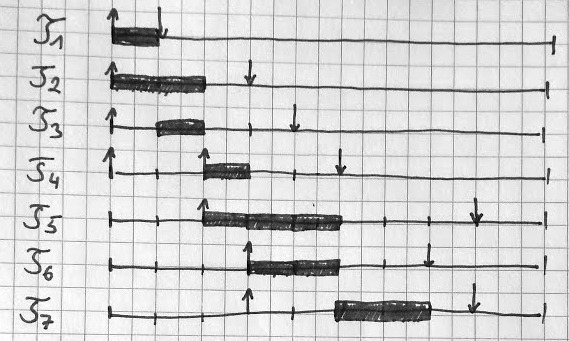
\includegraphics[scale = 2]{figures/c4_xi}\\
	\end{figure}
	\item The following table shows the slack times for each task $\Omega$ of  and each processor cycle.
	
	\begin{tabular}{ l | c | c | c | c | c | c | c | c | c}
  		\hline			
  		$\Omega$ & 1 & 2 & 3 & 4 & 5 & 6 & 7 \\
  		\hline
  		T1 & 2 	& 1 	& / 	& / 	& / 	& / & / \\
  		T2 & 1 	& 1 	& 1 	& 0 	& / 	& / & / \\
  		T3 & 3 	& 2 	& 1 	& 0 	& / 	& / & / \\
  		T4 & 1 	& 1 	& 0 	& 0 	& -1 	& -1 & / \\
  		T5 & (3) 	& 2 	& 1 	& 0 	& -1 	& / & / \\
  		T6 & (2) 	& 1 	& 0 	& 0 	& -1 	& -2 & / \\
  		\hline  
	\end{tabular}
	
	The resulting scheduling diagram:\\
	\begin{figure}[h]
	\centering
	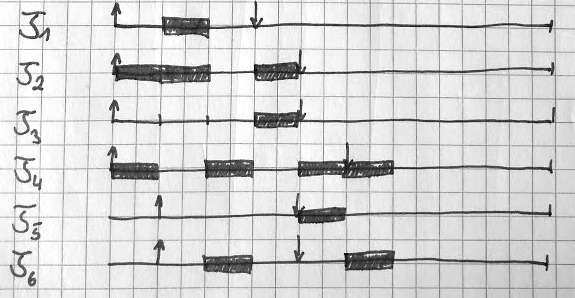
\includegraphics[scale = 2]{figures/c4_omega}\\
	\end{figure}
	
	As we can see, this set of tasks cannot be executed in a feasible schedule, even on a 2-core system.
	\end{itemize}
\end{itemize}

\end{document}
